% INTRODUCCIÓN

\cleardoublepage

\chapter{Introducción}
\label{introduccion}

Incluida en la clasificación de las bellas artes, en la lista propuesta por Ricciotto Canudo en su obra \emph{Manifiesto de las siete artes}, en la clasificación china de las tardes; y presente en cualquier obra audio visual contemporánea: cine, televisión, ``performances'', video juegos, ``video clips'', etc., la música es el elemento que marca una escena, condiciona una situación, acompaña una secuencia, potencia una acción, seduce a la audiencia, advierte al espectador o simplemente acompaña de fondo (y no por eso sin percibir menos atención) en la más mundana tarea como puede ser conducir un coche.

La música, en todos sus géneros formas, relata las costumbres de una región, de una nación, de un país, la moda de un determinado momento, se hace eco de hechos históricos y es capaz de transferir conocimiento y saber popular entre generaciones.

Es una manera de expresarse. Una forma de expresión que modifica la manera de sentir para seguir retroalimentando su presencia (quién no ha encontrado un patrón melódico en un llanto o en un ruido en plena calle).

La música, amplia, diversa e inmensa en número de piezas, consta de géneros musicales, que vienen a intentar clasificar y canonizar una composición musical, total o parcial, dentro de un grupo o conjunto, donde todos sus integrantes tengan rasgos comunes como: ritmo (compases y estructura), melodía, armonía, instrumentación, etc. En esencia, vienen a ser ``esas cosas que se perciben en conjunto y que hacen tipificar la pieza que se escucha''.

\section{Planteamiento del problema}

Tómese una serie de piezas musicales (cientos de ellas) y obténgase una representación computable de cada una. ¿Sería capaz una computadora de extraer patrones referenciales que permitieran clasificarlas? Esas clasificaciones: ¿se corresponderían con géneros musicales? ¿Cómo sabría la computadora de qué género musical se podría tratar en cada caso? Y si se añade una nueva pieza que concuerde levemente con alguna o algunas ya procesadas anteriormente, ¿será capaz de clasificarla? \textbf{¿Cómo aprende la máquina a distinguir géneros musicales?}

Esa es la gran pregunta que ha de hacerse para poder abordar la tarea de hacer un software que pueda clasificr piesas musicales.

... Y una vez clasificadas: \textbf{¿podría la máquina generar nuevas piezas musicales que se correspondan con un género conocido?}

Ese en concreto es el problema que se aborda en este trabajo de fin de máster. Para ello, se van a explorar distintas formas de abordar el problema, contraponiendo los resultados de unas y otras, y observando y evaluando qué alternativa cumple mejor con los requisitos planteados y cuál, además, aporta mejor gusto a la composición generada.


\section{Justificación}
(TODO: CONCRETAR JUSTIFICACIÓN CON YANETH)

\section{Objetivos}
\subsection{Principal}
\label{objetivo-principal}
Desarrollar un programa basado en Inteligencia Artificial que sea capaz de generar una pieza musical, que pueda clasificarse en un género concreto.

\subsection{Secundarios}

Para desarrollar el objetivo principal, han de cubrirse los objetivos secundarios:

\begin{itemize}
    \item Recopilar ejemplos de \textbf{datos} correspondientes con piezas musicales representativas, de un género músical y que estén \textbf{bien etiquetadas}.
    
    \item Transformar esas piezas musicales en \textbf{estructuras de datos} analizables y computables.

    \item Diseñar un modelo basado en Inteligencia Artificial que sea capaz de \textbf{extraer información} clave para \textbf{distinguir} cuáles son los \textbf{patrones} que asignan un pieza musical a un \textbf{género} concreto.

    \item Entrenar un modelo de Inteligencia Artificial, para que sea capaz de \textbf{generar} una pieza que sea reconocible como perteneciente a un género musical dado.

    \item \textbf{Evaluar} el modelo generador mediante métricas que se apliquen a los \textbf{datos de salida} generados. (TODO: VER MÉTRICAS)
\end{itemize}

\section{Alcance}
Si se atiende al objetivo principal~\ref{objetivo-principal}, el alcance viene dado por la cantidad de géneros a seleccionar para poder producir piezas musicales distintas. (Una pieza musical vendrá dada por un género y un ruido aleatorio introducido de manera automática, aspecto este que limitaría el número máximo de piezas musicales distintas a producir por el sistema; es por eso que este ruido habrá de ser de gran dimensión).

\section{Estructura del documento}
Este documento se organiza de la siguiente manera:
\begin{itemize}
    \item \emph{Capítulo \textbf{1}}\textbf{: Introducción.} Presentación, exposición del problema y del trabajo que lo intenta resolver, justificación, objetivos, alacance y estructura (esta misma sección).
    \item \emph{Capítulo \textbf{2}}\textbf{: Estado del arte.} Revisión exhaustiva del estado del arte en el momento de acometer este trabajo fin de máster.
    \item \emph{Capítulo \textbf{3}}\textbf{: Marco teórico.} Exposición de los fundamentos teóricos en los que se basa este trabajo.
    \item \emph{Capítulo \textbf{4}}\textbf{: Métodos y Materiales.} Metodología utilizada y herramientas para llevar a cabo todo el proceso proyectual.
    \item \emph{Capítulo \textbf{5}}\textbf{: Resultados y Análisis.} Contraste de resultados y análisis de los mismos.
    \item \emph{Capítulo \textbf{6}}\textbf{: Conclusiones.} Presentación de conclusiones obtenidas del producto global del trabajo.
    \item \emph{Capítulo \textbf{7}}\textbf{: Limitaciones y perspectivas a futuro.} Propuestas de mejoras y líneas de expansión para futuros trabajos.
\end{itemize}

\textbf{Esta palabra} está en negrita. \textit{Esta palabra} está en cursiva. \destacado{Esta palabra} se destaca en púrpura.
\medskip

\section{Mi segunda sección}
\label{mi-segunda-seccion}

En la sección~\ref{mi-primera-seccion} se muestran ejemplos de palabras en negrita, cursiva y destacadas en púrpura.
\medskip

% Define los acrónimos en el fichero secciones/glosario.tex
% Define la bibliografía en el fichero bibliografia.bib
Una \acrfull{gan} es... \citep{goodfellow2014generative}.
\medskip

\citet{goodfellow2014generative} diseñaron las redes generativas antagónicas como...
\medskip

\vspace{5ex}

Listado:
\begin{itemize}
  \item Item 1.
  \item Item 2.
  \item Item 3.
\end{itemize}

Enumeración:
\begin{enumerate}
  \item Item 1.
  \item Item 2.
  \item Item 3.
\end{enumerate}

\subsection{Una subsección}
\label{una-subseccion}

La figura~\ref{fig1} muestra...

\begin{figure}[ht!]
    \centering
    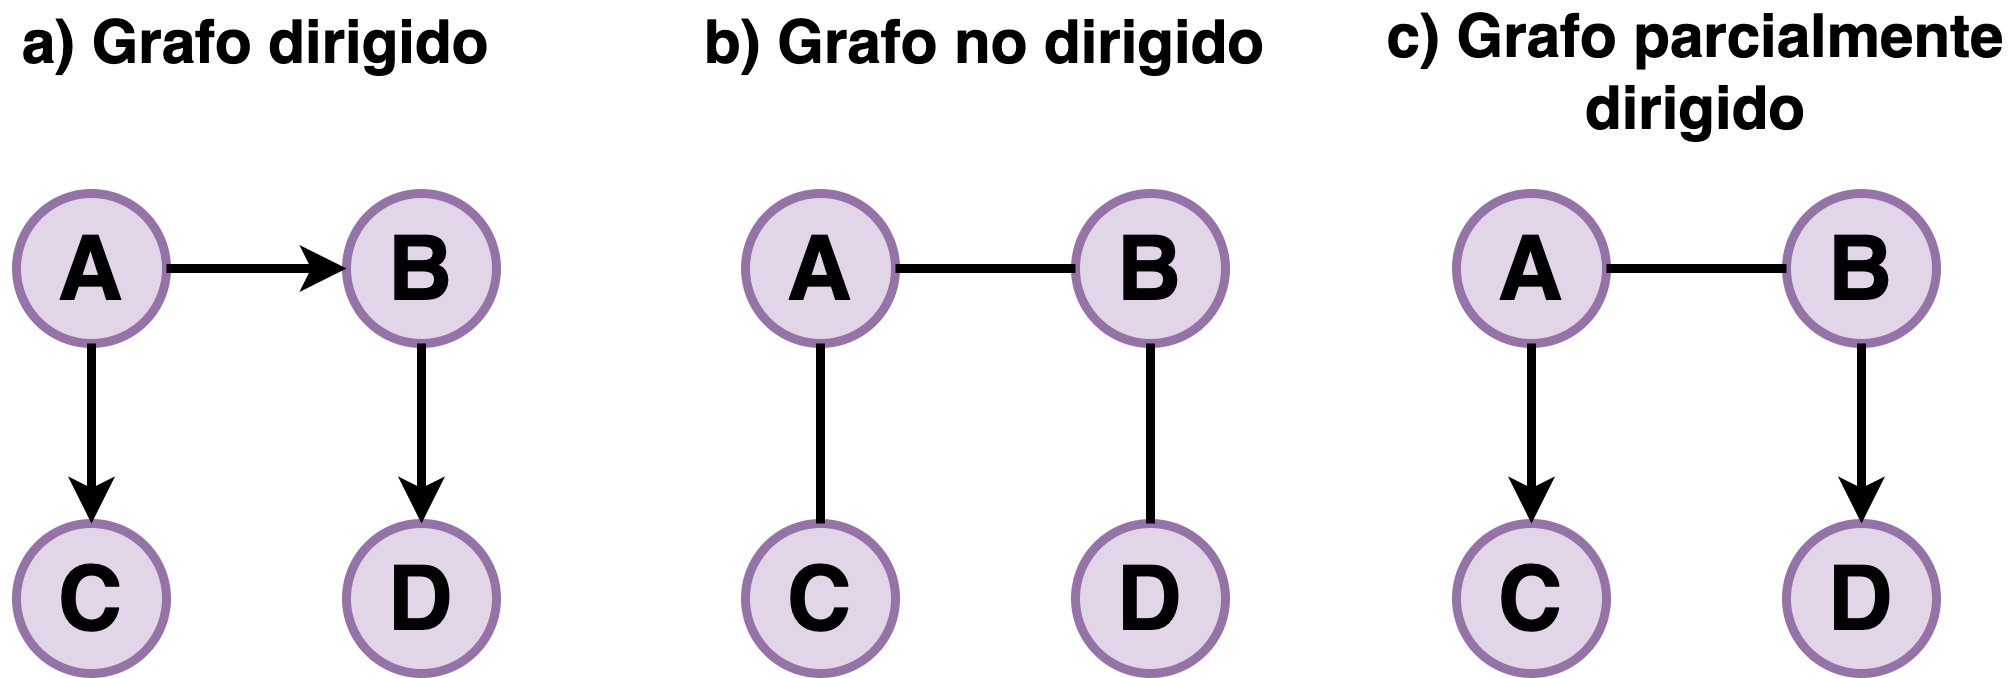
\includegraphics[scale=0.15]{figuras/fig1.png}
    % \caption[Así aparece el rótulo en el índice]{Así aparece el rótulo en el texto.}
    \caption[Tipos de grafos]{\textbf{Tipos de grafos.}}
    \label{fig1}
\end{figure}

La tabla~\ref{tab1} muestra...

\begin{table}[H]
    \centering
    \caption{Resumen de documentos y arquitecturas en el estado del arte}   
    \resizebox{0.95\textwidth}{!}{%
    \begin{tabular}{|p{2cm}|c|c|c|c|c|p{4.3cm}|p{5.6cm}|c|c|}
        \hline
        \rowcolor{gray!20} \textbf{Documento} & \textbf{CNN} & \textbf{VAE} & \textbf{GANs} & \textbf{Transformers} & \textbf{LSTM} & \textbf{Aplicación en la Música} & \textbf{Relevancia en el Estado del Arte} & \textbf{Simbólica} & \textbf{Audio} \\
        \hline
        \textbf{TFG Antonio Carpintero Castilla} & \ding{51} & \cellcolor{red!25} & \cellcolor{red!25} & \cellcolor{red!25} & \ding{51} & Generación de música Lo-Fi & Caso práctico en generación de un género específico & \ding{51} & \cellcolor{red!25} \\
        \hline
        \textbf{Estado del Arte - M72.1.09 Gestión y análisis de datos no estructurados} &  & \cellcolor{red!25} & \cellcolor{green!25}\ding{51} & \cellcolor{green!25}\ding{51} &  & Modelado de datos en entornos no estructurados & Explica el papel de Transformers en la IA musical & \ding{51} & \cellcolor{red!25} \\
        \hline
        \textbf{AI of Things (VI) - Inteligencia Artificial Generativa, creando música a ritmo de perceptrón} &  & \cellcolor{green!25}\ding{51} & \cellcolor{green!25}\ding{51} & \cellcolor{red!25} &  & Aplicación de modelos generativos en la música & Explica GANs y VAE en la síntesis musical & \ding{51} & \cellcolor{red!25} \\
        \hline
        \textbf{IA en la creatividad: Explorando la generación de arte y música} &  & \cellcolor{green!25}\ding{51} & \cellcolor{green!25}\ding{51} & \cellcolor{red!25} &  & Modelos generativos aplicados al arte y música & Justificación del impacto de la IA en la música &  & \cellcolor{green!25}\ding{51} \\
        \hline
        \textbf{A Transformer Generative Adversarial Network for Multi-Track Music Generation} &  & \cellcolor{red!25} & \cellcolor{green!25}\ding{51} & \cellcolor{green!25}\ding{51} &  & Generación de música polifónica multicanal & Combinación de Transformers y GANs para mejorar generación & \ding{51} & \cellcolor{red!25} \\
        \hline
        \hline
        \textbf{TFM} &  & \cellcolor{blue!25}\ding{51} & \cellcolor{blue!25}\ding{51} & \cellcolor{blue!25}\ding{51} &  & Generación de música personalizada & Justificación de modelos generativos en el TFM & & \cellcolor{blue!25}\ding{51} \\
        \hline
    \end{tabular}%
    }
    \label{tab1}
\end{table}

\subsection{Una subsubsección}
\label{una-subsubseccion}

El algoritmo~\ref{alg1} muestra...
\medskip

\begin{algorithm}[H]
\label{alg1}
\SetAlgoLined
\medskip
\begin{enumerate}
    \item Elegir una estructura de red $\mathcal{G}$ sobre $\mathbf{V}$, normalmente vacía. Establecer la puntuación máxima inicial: $Score_{max} = Score_{\mathcal{G}}$.
    \item Repetir los siguientes pasos mientras $Score_{max}$ siga aumentando:
    \begin{enumerate}
        \item Calcular las puntuaciones para todas las posibles redes modificadas $\mathcal{G}^{*}$ que se pueden obtener añadiendo, eliminando o reorientando un solo eje de $\mathcal{G}$ sin que se producan ciclos.
        \item Si para alguna de las redes modificadas $\mathcal{G}^{*}$ se cumple que $Score_{G^{*}} > Score_{\mathcal{G}}$, establecer $G = G^{*}$ y $Score_{max} = Score_{G^{*}}$.
    \end{enumerate}
    \item Devolver el DAG $\mathcal{G}$.
\end{enumerate}
 \caption{Algoritmo \textit{Hill-Climbing} (HC)}
\end{algorithm}


\newpage

Ejemplo de fórmula:

\begin{equation*}
    N_{k}(\mathbf{\mu},\mathbf{\Sigma}) = \frac{1}{\sqrt{2\pi\det(\Sigma})} \exp \bigg\{ -\frac{1}{2}(\mathbf{X}-\mathbf{\mu})^{T}\Sigma^{-1}(\mathbf{X}-\mathbf{\mu}) \bigg\} \quad \mathbf{X},\mathbf{\mu} \in \mathbb{R}^{k}
\end{equation*}

Otro ejemplo de fórmula:

\begin{equation*}
    \underbrace{P(\mathcal{B}|\mathcal{D}) = P(\mathcal{\mathcal{G}},\Theta|\mathcal{D})}_{\textbf{Aprendizaje}} = \underbrace{P(\mathcal{G}|\mathcal{D})}_{\textbf{Aprendizaje estructural}} \cdot \underbrace{P(\Theta|\mathcal{G},\mathcal{D})}_{\textbf{Aprendizaje paramétrico}}
\end{equation*}
